%roughly 2-3 pages
%\begin{itemize}
%\item explain the model; if any important assumptions are made at this stage, explain why they are reasonable or necessary
%\item Explain learning / inference algorithms
%\item explaining (perhaps briefly) any necessary preprocessing/postprocessing data acquisition stages (maybe earlier, depending on the project; may also move to the experimental section)
%\end{itemize}
\subsection{Extended LDA model}
Latent Dirichlet Allocation (LDA) treats every document like a collection of words, and presumes that each word in a document is generated by a certain topic. A hidden distribution over topics is assumed to exist for every document. The goal of LDA is to \textit{a)} find a distribution over topics for each document and \textit{b)} find a distribution over words for each topic. Thus, we're looking for two sets of distributions: $\theta_i \sim \text{Dirichlet}(\alpha)$, or a distribution of topics over document $i$, and $\varphi_k \sim \text{Dirichlet}(\beta)$, or a distribution of words over topic $k$. Thus, LDA assumes that some generative model generates a document: for each word position $i,j$ from $i \in$ documents and $j \in$ words$_i$, choose a topic $z_{ij} \sim \theta_i$, then choose a word $w_{ij} \sim \varphi_{z_{ij}}$. \\
In this paper, LDA is extended: instead of finding distributions over topics for every document, topic distributions are learned over genres, where a genre is a non-overlapping set of documents. The difference between regular LDA and genre-LDA can be seen in the graphical models found in figure \ref{fig:graphical-model} (original LDA) and \ref{fig:graphical-model_extended} (genre-LDA). \\
To infer the different distributions, collapsed Gibbs sampling is used (where the distributions $\theta_i$ and $\varphi_k$ are integrated out). The derivation for genre-LDA is similar to, but not exactly the same as the derivation for original LDA. The derivation can be found in section \ref{ref:derivation}.\\

\begin{figure}[htp]
	\centering
	\begin{subfigure}[b]{0.5\textwidth}
		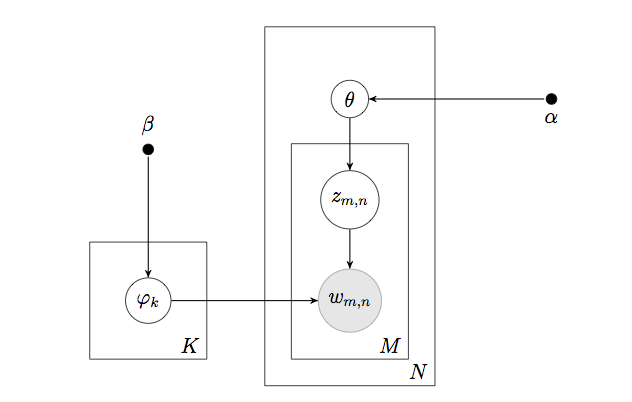
\includegraphics[width=\textwidth]{regular_lda_img}
		\caption{Graphical model for regular LDA}
		\label{fig:graphical-model}
	\end{subfigure}%
        \begin{subfigure}[b]{0.5\textwidth}
		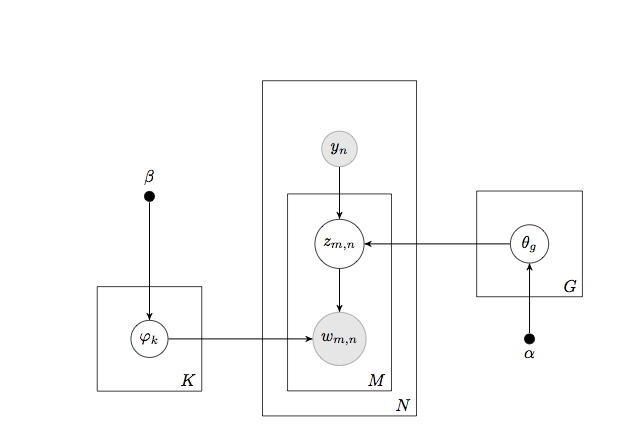
\includegraphics[width=\textwidth]{extended_lda_img}
		\caption{Graphical model for extended LDA}
		\label{fig:graphical-model_extended}
	\end{subfigure}
\end{figure}

\subsubsection{Gibbs sampling}
The calculation of the total probability of the model is computationally difficult because it marginalizes by integrating over a joint distribution. Therefore, the collapsed Gibbs sampling algorithm is applied for the (extended) LDA model. This algorithm samples from a conditional distribution which asymptotically approaches the correct distributions and is computationally simple compared to the marginalization of the total probability. The formula for the conditional probability used in Gibbs sampling algorithm for the extended LDA model can be found in section \ref{ref:derivation}. As can be seen in this formula, the conditional probability is also dependent on the counts of topics that occur in documents with the same genre instead of only the document in question.

\begin{mdframed}
\begin{algorithm}[H]\label{alg:create-song}
 \KwData{Topic Model inferred by extended DA, genre $G$, number of documents $N$, words in document i $M_i$}
 \KwResult{word-topic and topic-genre distribution}
\textbf{Initialize:} randomly assign words to topics \\
 assign topics to genre given genre of doc in which word is found\\
 \For{ Document $i$ where $i\in 1\dots N$ }{
 	\For{word $j$ where $j\in 1\dots M_i$}{
  calculate conditional probability distribution for $z_{i,j}$\\
  sample topic from distribution $k$\\
  update word-topic distrubtion given $z_{ij} = k$\\
  update topic-genre distrubtion given $G$\\
	}
 }
 return word-topic distribution, topic-genre distribution
 \caption{Gibbs sampling for extended LDA}
\end{algorithm}
\end{mdframed}
 

\subsubsection{Generative model}
Since LDA is a generative model, it can also be used to create new lyrics. To create a `song' of length $n$ for a genre $G$, for each word position from $0$ to $n$, a topic $k$ is sampled from $G$'s topic distribution. Then, a word is sampled from $k$'s word distribution (see also algorithm \ref{alg:create-song}). \\
\begin{mdframed}
\begin{algorithm}[H]\label{alg:create-song}
 \KwData{Topic Model inferred by extended LDA, genre $G$, length $n$}
 \KwResult{Song for genre $G$ of length $n$}
 initialize: song = `' \\
 \While{counter $< n$ }{
  sample $k \sim \theta_G$\\
  sample $w \sim \varphi_k$\\
  append $w$ to song\\
  counter ++ \
 }
 return song
 \caption{Song generation}
\end{algorithm}
\end{mdframed}

\subsection{Data acquisition}
Before any model could be tested, data had to be collected and processed. To do this, a crawler was built that collects song lyrics from \textit{Lyricsmode}\footnote{\texttt{http://www.lyricsmode.com}} by going through the alphabet (with one `letter' for numbers $0-9$), finding the top 100 artists starting with that letter and collecting the first five songs (alphabetically) by that artist. After collecting these lyrics, genre-information was retrieved from \textit{Allmusic}\footnote{\texttt{http://www.allmusic.com}}. The choice of these websites are primarily based on earlier research \cite{felllyrics} that used these websites because of their consistency. \\
After collecting a dataset of $12.102$ lyrics, the data was pre-processed to filter out \textit{a)} punctuation marks and capitalization \textit{b)} non-english lyrics and \textit{c)} low-content, very common words\footnote{For example, 'a', 'by', 'I', 'off', 'were'}, resulting in a dataset of $9.728$ lyrics. These pre-processing steps were done under the assumption that for topic modeling, including common words would create low-information topics that would hardly contribute to the model. Another assumption was made that punctuation and capitalization, while containing useful information regarding language, were not relevant to the kinds of topics that would be found (as topic modeling is usually a bag-of-words approach). Non-english lyrics were filtered because extraction topics over multiple language would add a lot of noise to the model. Note however, that not \textit{all} non-english words were filtered out (only complete songs in a different language): in many cases, the use of \textit{some} non-english words can say a lot about a genre\footnote{Think of the Latin genre, for example, which turned out to use both english and spanish words quite a lot}. 




